\subsection{The TorPath Protocol}

\subsubsection{Overview}

The TorPath protocol assigns Tor circuits to clients, overriding Tor directory
servers with \textit{assignment servers}, which form decentralized
\textit{consensus groups}. The protocol guarantees that no participant on a
circuit can identify all other participants, and that each circuit includes a
publicly verifiable signature. We use TorPath to ``sign'' each TorCoin, so
that anyone can blindly verify a TorCoin by comparing its signature to a
global circuit history.

\subsubsection{Requirements}

The TorPath protocol adheres to the following constraints:

\begin{itemize}   
\item No client can generate its own circuit.
\item Every circuit has a unique, publicly-verifiable signature.
\item No client can know the circuit of another client.
\end{itemize}

A consensus group is formed when a majority of the Assignment Servers come
together to assign circuits to clients. Thus, if there are 10 Assignment
Servers in the network, atleast 6 of them must collectively form a group.  The
size of each anonymity group can be modulated to be a number n, i.e., the
group waits until there are n clients to proceed to the next stage. Different
groups can have different values of n to allow each client to choose its own
anonymity level different levels of anonymity. Groups with larger values of n
would provide a larger anonymity set, at the expense of longer circuit setup
times.

\subsubsection{Protocol Description}

The protocol consists of three sequential steps:

\begin{enumerate}
\item \textbf{Group Initialization.} Assignment servers form a \textit{consensus group} by exchanging the public keys of all clients and relays connected to them. 
\item \textbf{Verifiable Shuffle.} The consensus group performs a decentralized, 
verifiable shuffle of all the public keys, resulting in a circuit assignment for
each client.
\item \textbf{Path Lookup.} The assignment servers publish the result of the 
shuffle, such that each client can only identify its entry relay, and each relay
can only identify its neighbors. 
\end{enumerate}


\paragraph{(1/3) Group Initialization}

When a majority of the assignment servers have a sufficient number $n$ of
clients and relays connected to them, they form a consensus group. Clients and
relays can specify a minimum $n$ required to join a consensus group. A larger
$n$ results in a larger anonymity set, but slower connection speeds while
assignment servers wait for more clients and relays to come online.

A consensus group forms in three separate steps:

\begin{enumerate} 

\item \textbf{Each assignment server} shares its public key with its group
members, and broadcasts the public keys it receives to all clients and relays
connected to it.

\item \textbf{Each client} generates a temporary private and public key pair.
It uses ``onion encryption'' to combine its public key with the public keys of
all assignment servers in the group, resulting in a hash that each server can
only partially decrypt. It sends this hash to its own server.

\item \textbf{Each relay} can act as an entry, middle, and/or exit relay, and
it chooses which position(s) to assume. In most cases, the number of available
relays will be less than that of clients in a group. To ensure parity between
clients and relays for each position, each assignment server instructs its relays to generate a
sufficient number of keys for each position. The relay server uses
onion-encryption to generate $n$ cipher-texts from $n$ temporary public keys.
It packages them by position and sends them to its assignment server.
\end{enumerate}

Figure \ref{figure:transfer} illustrates Steps 2 and 3, after the assignment
servers exchange public keys.

\begin{figure}[htbp]
  \centering
  \subfloat[]{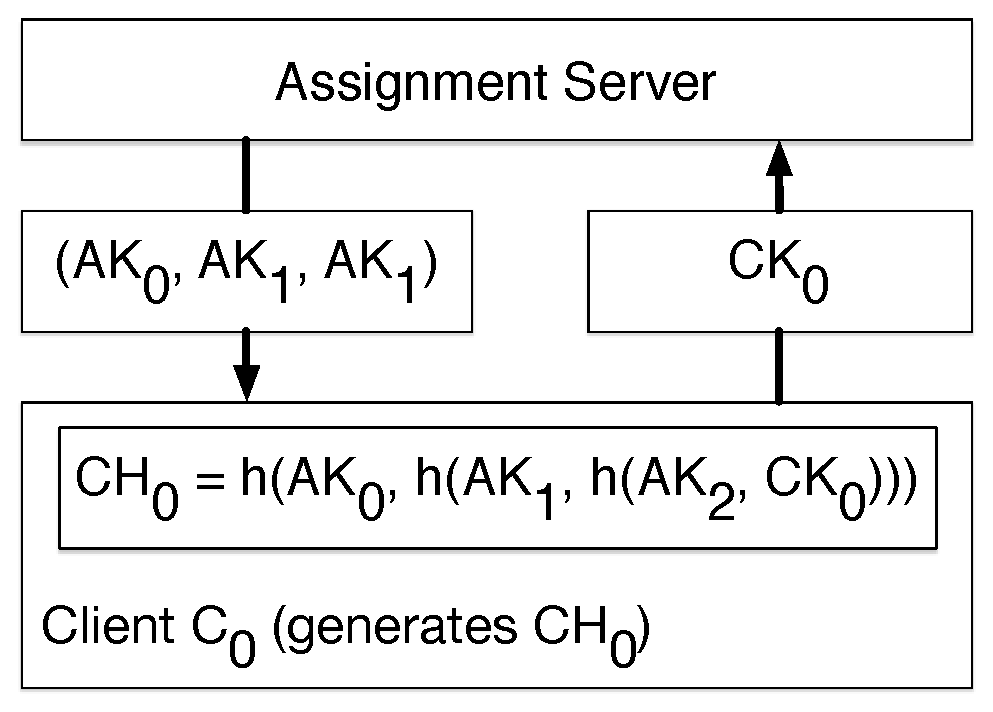
\includegraphics[width=.49\textwidth]{group_formation_2.pdf}}
  \subfloat[]{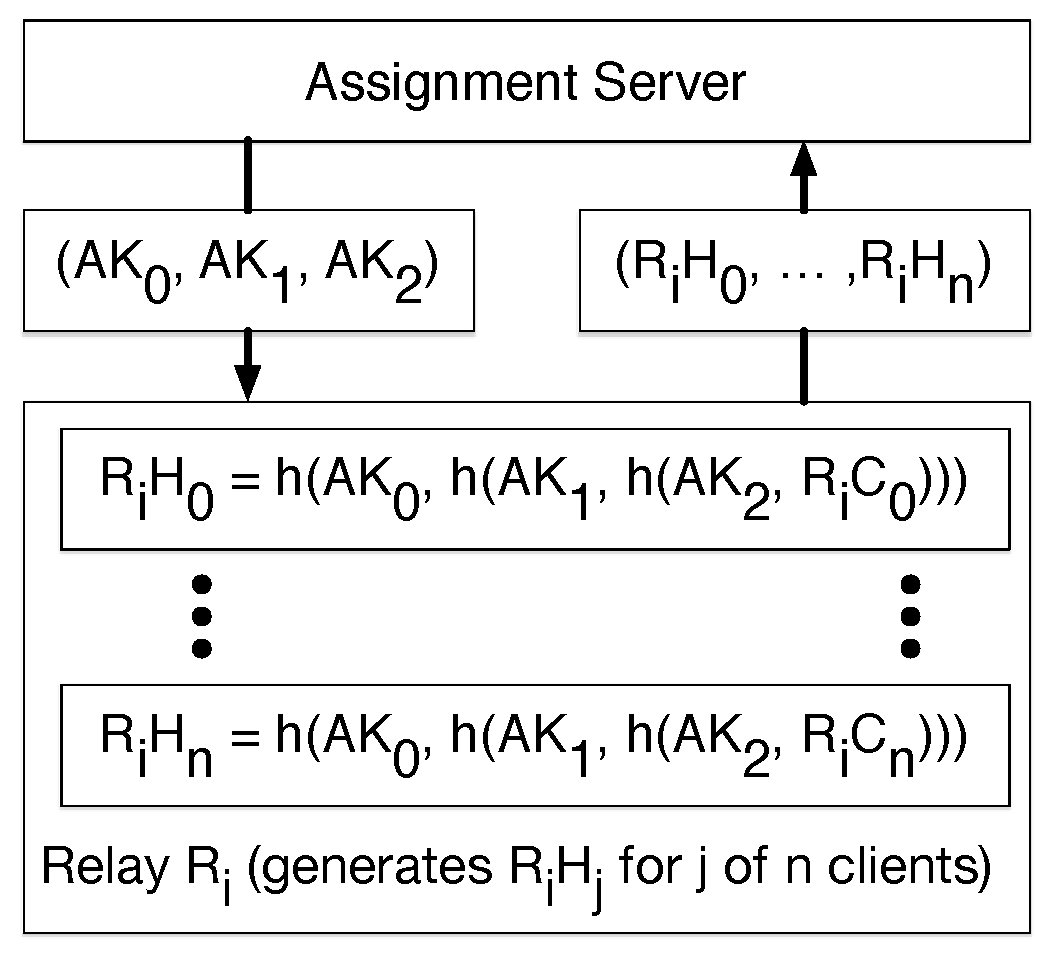
\includegraphics[width=.49\textwidth]{group_formation_3.pdf}}
  
  \caption{Both relays and clients use onion-encryption to combine their own
  temporary public keys with the public keys of all assignment servers in the group. (a) Client generates one hash. (b) Each relay generates an onion hash for $n$ clients, as instructed by assignment servers, and decides on a position
  for each client.}
  \label{figure:transfer}
\end{figure}

We can represent the list of keys as a $4 \times n$ matrix $M$ for $n$
clients, where each row corresponds to a client and its three relays (see
Figure \ref{figure:shuffle}).

\paragraph{(2/3) Verifiable Shuffle} The assignment servers now ``shuffle''
each column so that each client row contains a random triple of relay public
keys. The consensus group collectively shuffles the columns using a verifiable
shuffling algorithm, like the Neff Shuffle \cite{neff2001verifiable}.


\begin{figure}
  \centering
    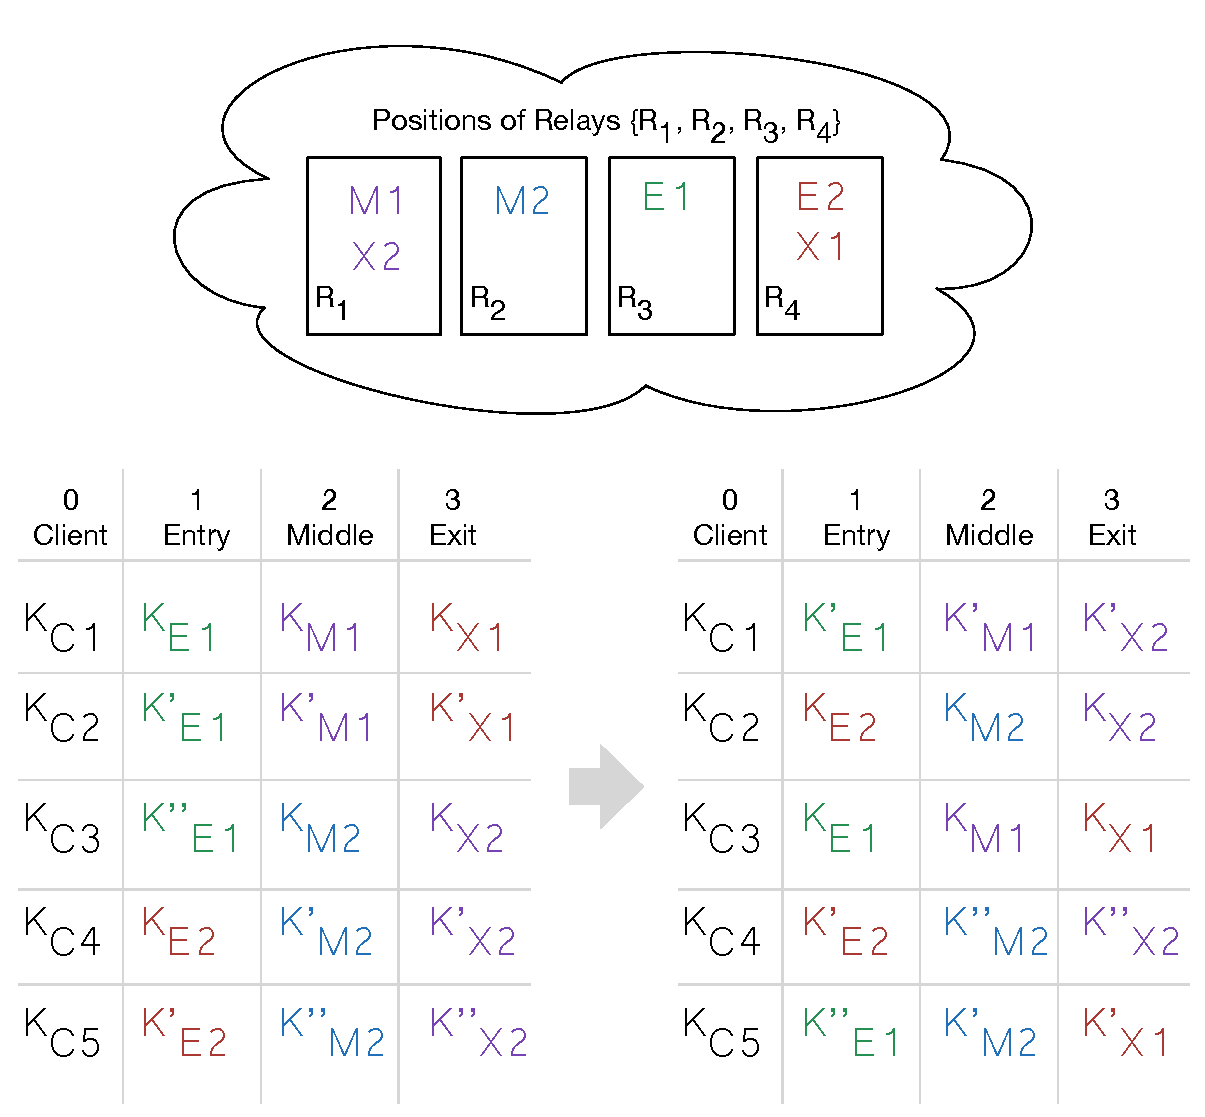
\includegraphics[scale=.6]{shuffle_total.pdf}
  \caption{Example matrix shuffle with 5 clients ($C_1$, $C_2$, $C_3$, $C_4$ and $C_5$) and 4
relays (Purple, Blue,Green, Red). There are two entry relays (Green and Red),
two middle relays (Purple and Blue) and two exit relays (Purple and Red). Each
row $i$ contains the public keys of a client $K_{Ci}$ and three relay positions
$(K_{Ei}, K_{Mi}, K_{Xi})$. The group of assignment servers collectively shuffles
the matrix so that each row represents a circuit.}
  \label{figure:shuffle}
\end{figure}


The assignment servers collectively sign and publish the resulting matrix to a
public log, accessible by all clients and relays.

\paragraph{(3/3) Path Lookup}
Path lookup is the final step of the algorithm, where each client obtains the
IP address of its entry relay, and each relay obtains the IP address of its
neighbor(s) on the circuit. The path lookup algorithm ensures that each client
and relay can only receive the IP address of its circuit neighbors.

Each client encrypts its own IP using the public key of its neighbor. It then
creates a tuple of the form (public key, encrypted IP) as described in table
\ref{table:message_format}. This tuple is then onion-encrypted and sent to the
server.  Each relay also follows the same procedure, but for every key in the
matrix that belongs to it.

The assignment servers shuffle this new list of tuples. At this point, each
client and relay can find its neighbors in the matrix by locating the tuples
containing the public keys it needs. Finally, it decrypts those cells using
its private key, revealing the IP address of its circuit neighbor(s).

Now clients have a circuit they can use for Tor.

{\renewcommand{\arraystretch}{2}
\begin{table}[h]
\centering
  \begin{tabular}{ |c || c| }
  \hline
  \textbf{Sender} & \textbf{Message Tuple} \\ \hline
  Client & ($K_{i}^{C}$, $\{IP_{i}^{C}\}_{K_{i}^{E}}$) \\ \hline
  Entry relay & ($K_{i}^{E}$, $\{IP_{i}^{E}\}_{K_{i}^{C}}$, $\{IP_{i}^{E}\}_{K_{i}^{M}}$) \\ \hline
  Middle relay & ($K_{i}^{M}$, $\{IP_{i}^{M}\}_{K_{i}^{E}}$, $\{IP_{i}^{M}\}_{K_{i}^{X}}$) \\ \hline
  Exit relay & ($K_{i}^{X}$, $\{IP_{i}^{X}\}_{K_{i}^{M}}$) \\ \hline
  \end{tabular}
  \caption{Each participant in a circuit sends its message 
  tuple onion-encrypted to the server. $\{X\}_{Y}$ denotes X being encrypted with Y.}
  \label{table:message_format}
\end{table}

\paragraph{Circuit Signature} The Circuit Signature of the $i^{th}$ circuit in
a shuffle is an ordered pair consisting of the hash of the matrix M and the
row number of the circuit in the matrix M: $CS_i = (Hash(M), i)$. This
signature will be used in the TorCoin algorithm to prove that TorCoins are
minted only by circuits that have been assigned by consensus groups.

\subsection{Security Considerations} 

\subsubsection{Anonymity} The TorPath protocol guarantees that no single
server can be aware of the entire circuit of any client. If there are malicious
colluding clients or relays, they will be able to shrink the anonymity set to
the set of honest relays and clients in the consensus group.  Groups have
various sizes, allowing clients to choose the anonymity threshold they
require.

\subsubsection{Random Group Selection} The TorPath protocol increases
robustness of TorCoin to attackers. Its random group selection system prevents
attackers from deterministically placing themselves in a group. We assume that
atleast one of the assignment servers in the group is honest. In this case,
the group as a whole is able to retain privacy and anonymity. We could make
the system even more secure by randomizing group assignment, instead of just
taking temporal locality to be the only criterion.

\subsubsection{Same relay in multiple positions}  It is possible that through
a Neff shuffle, the same relay gets assigned to a circuit in multiple
positions (Eg. The same physical relay could be both the entry and middle
relays.) This does not pose a challenge as it is analogous to a Tor client
choosing multiple relays owned by the same operator.


% % Next we will descibe the consensus groups and Neff shuffle in more detail.

% % \begin{figure}[H] %   \centering %
% 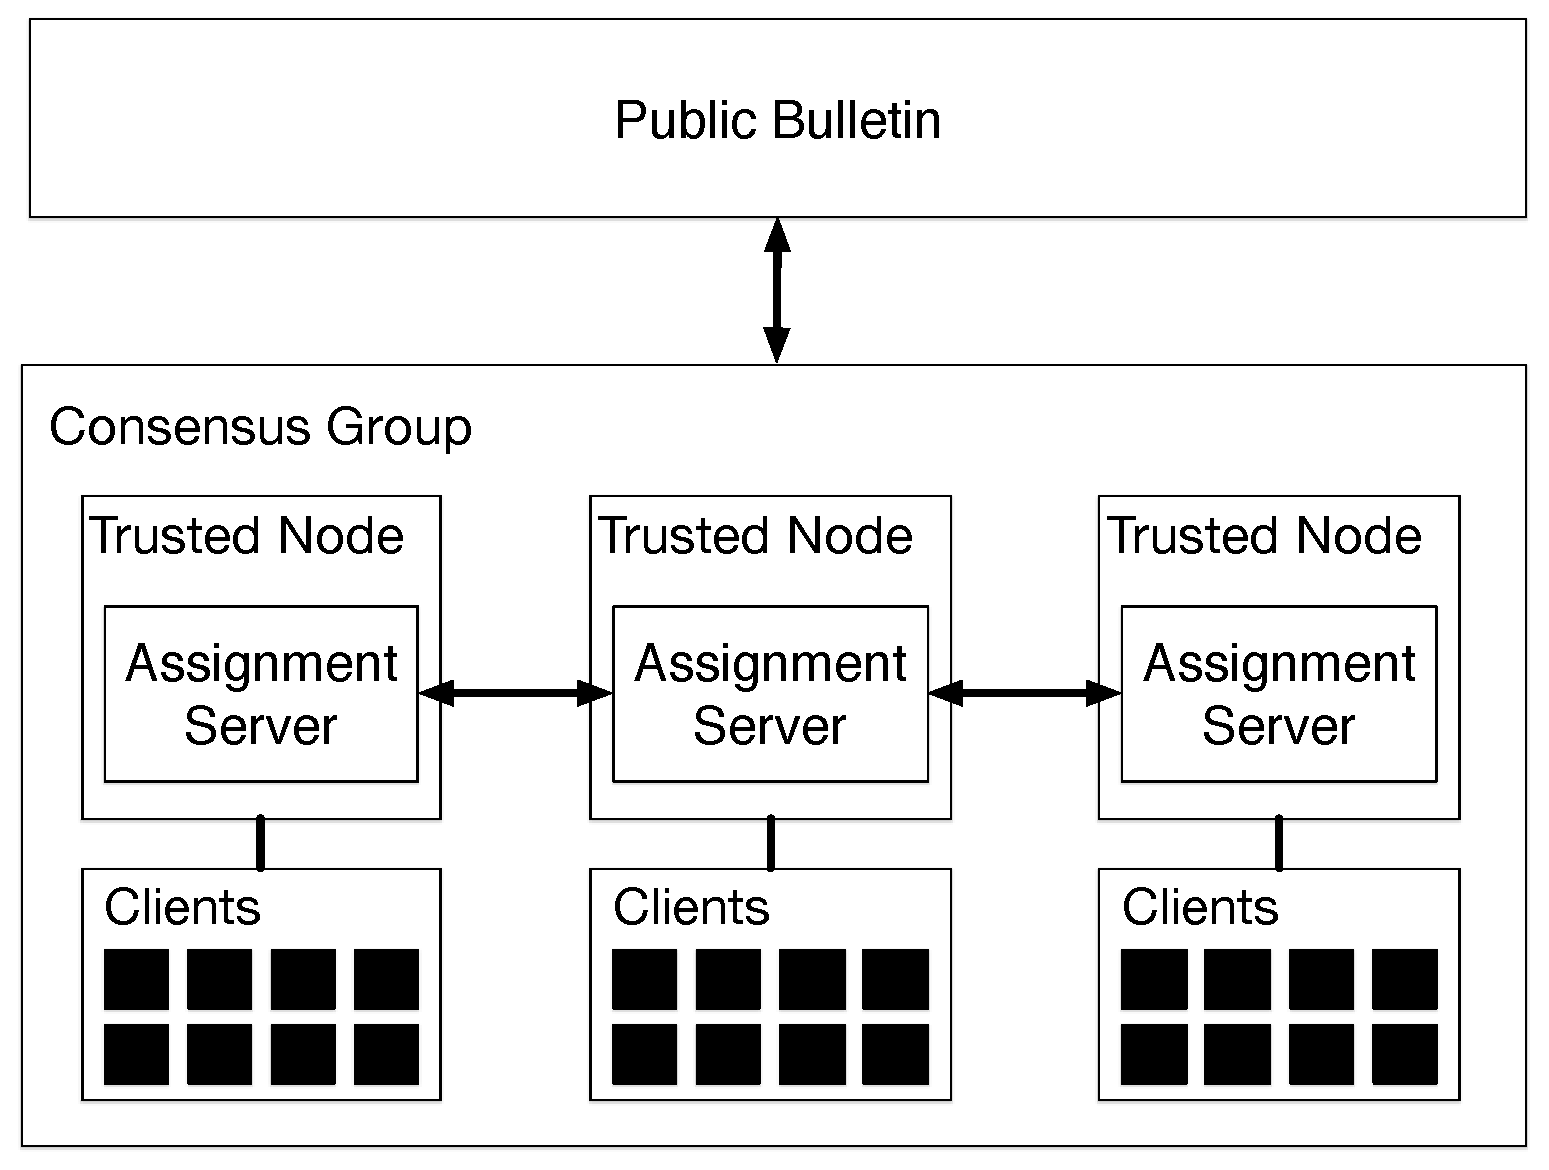
\includegraphics[scale=0.3]{torpath_grouping.pdf} %   \caption{TorPath Consensus
% Group Formation.} % \end{figure}

% % \subsubsection{Group Formation} % An assignment server joins a group when it
% reaches a sufficient number of clients. In practice, we expect the number to be
% modulated so that groups are being created every 10 seconds or so. To ensure
% diversity, groups must include a majority of the assignment servers on the
% network. For example, if there are ten of assignment servers on the entire
% network, a consensus group requires at least six.

% % Once a consensus group exists, it splits into three decentralized shuffle
% % sets, each responsible for assigning a different relay to clients. An
% % $n$-client shuffle set has $n$ rows, each pointing to a possible relay. For
% % example, shuffle sets $s_0$, $s_1$, and $s_2$ could be responsible for
% % assigning entry, middle, and exit relays to clients.

% % \subsubsection{Neff Shuffles for Circuit Assignment} % Each shuffle set runs a
% Neff shuffle ~\cite{neff2001verifiable} to shuffle its list of $n$ relays, so
% that it can assign each relay $i$ to client $i$. Each client receives a tuple
% $(r_0, r_1, r_2, s)$ specifying the address of entry, middle, and exit relays,
% along with a circuit signature.

% % \begin{figure} %   \centering %
% 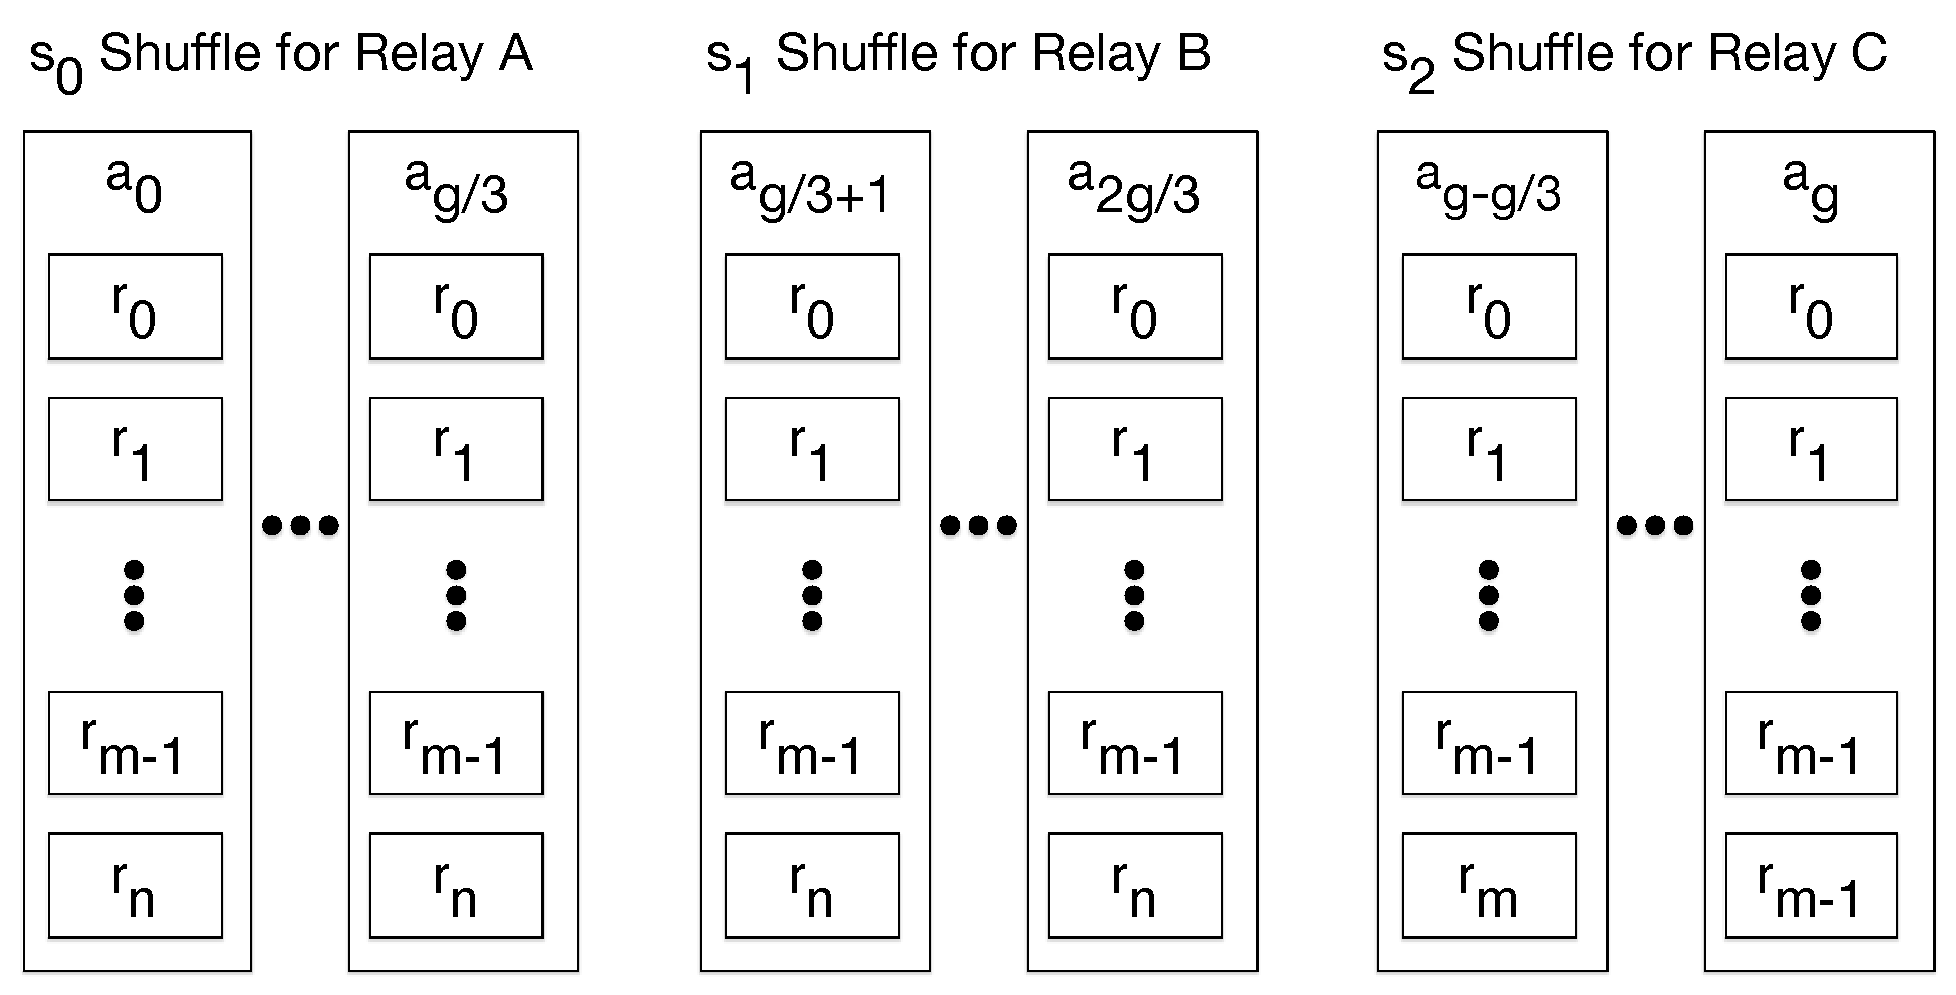
\includegraphics[scale=0.3]{torpath_shufflesets.pdf} %   \caption{Each Shuffle
% Set carries out its own Neff shuffle to determine one part of the path.} %
% \end{figure}

% % \subsubsection{TorCoin Verification} % Assignment servers input circuit
% signatures into a cryptographic accumulator, and publish that list of
% accumulators. Anyone can verify that a circuit existed at least once, simply by
% searching for a signature.

% % \subsubsection{Decoupled Protocol} % The TorPath protocol only replaces
% directory servers. Therefore, implementing it does not require modifying any Tor
% code. So clients can use the TorPath protocol for circuit assignment then
% communicate using the existing Tor protocol.
